%%%%%%%%%%%%%%%%%%%%%%%%%%%%%%%%%%%%%%%%%%%%%%%%%%%%%%%%%%%%%%%%%%%%%%%%%%%%
% AGUJournalTemplate.tex: this template file is for articles formatted with LaTeX
%
% This file includes commands and instructions
% given in the order necessary to produce a final output that will
% satisfy AGU requirements, including customized APA reference formatting.
%
% You may copy this file and give it your
% article name, and enter your text.
%
%
% Step 1: Set the \documentclass
%
%

%% To submit your paper:
\documentclass[draft]{agujournal2019}
\usepackage{url} %this package should fix any errors with URLs in refs.
\usepackage{lineno}
\usepackage[inline]{trackchanges} %for better track changes. finalnew option will compile document with changes incorporated.
\usepackage{soul}
\linenumbers
%%%%%%%
% As of 2018 we recommend use of the TrackChanges package to mark revisions.
% The trackchanges package adds five new LaTeX commands:
%
%  \note[editor]{The note}
%  \annote[editor]{Text to annotate}{The note}
%  \add[editor]{Text to add}
%  \remove[editor]{Text to remove}
%  \change[editor]{Text to remove}{Text to add}
%
% complete documentation is here: http://trackchanges.sourceforge.net/
%%%%%%%

%\draftfalse

%% Enter journal name below.
%% Choose from this list of Journals:
%
% JGR: Atmospheres
% JGR: Biogeosciences
% JGR: Earth Surface
% JGR: Oceans
% JGR: Planets
% JGR: Solid Earth
% JGR: Space Physics
% Global Biogeochemical Cycles
% Geophysical Research Letters
% Paleoceanography and Paleoclimatology
% Radio Science
% Reviews of Geophysics
% Tectonics
% Space Weather
% Water Resources Research
% Geochemistry, Geophysics, Geosystems
% Journal of Advances in Modeling Earth Systems (JAMES)
% Earth's Future
% Earth and Space Science
% Geohealth
%
% ie, \journalname{Water Resources Research}


% 12 Publication Units (500 words or one figure)
% 1 Table: list of distributions
% 2 Image: illustration of orientation
% 3 Image (appendix): multi-panel comparison of performance
% 4 Image distributions (filtered, sheltered/unsheltered)
% 5 image standard deviation and wind


\journalname{JGR: Atmospheres}


\begin{document}

\title{Observation of the orientation  of snow hydrometeors at sheltered and unsheltered sites}

\authors{J. Grazioli\affil{1}, M. Condolf\affil{2}, Y.-A. Roulet\affil{3} F. Coletti\affil{2}, and A. Berne\affil{1}  }

\affiliation{1}{Environmental Remote Sensing Laboratory, École Polytechnique Fédérale de Lausanne, Lausanne, Switzerland}
\affiliation{2}{Department of Mechanical and Process Engineering, ETH, Zürich, Switzerland}
\affiliation{3}{Swiss Federal Office of Meteorology and Climatology (MeteoSwiss)}

\correspondingauthor{Jacopo Grazioli}{jacopo.grazioli@epfl.ch}

%% Keypoints, final entry on title page.

%  List up to three key points (at least one is required)
%  Key Points summarize the main points and conclusions of the article
%  Each must be 140 characters or fewer with no special characters or punctuation and must be complete sentences

\begin{keypoints}
\item Observations of snowflake orientations show symmetrical distributions around 0$^\circ$ and standard deviations that confirm some of the assumptions made in theoretical studies. 
\item Sheltered and unsheltered sites show systematic differences in orientation distributions. Instrument (local perturbations) and atmospheric effects cannot be separated.
\item Numerical simulations reveal that common estimation choices made in past studies may lead to data processing artifacts.
\end{keypoints}



\begin{abstract}
Knowledge about orientation of falling snow is still poorly documented with field measurements despite its importance, for example, in the interpretation of remote sensing data. This study investigates the orientation of snow hydrometeors using data from a Multi-Angle Snowflake Camera (MASC). We explore the impact of different observational setups (sheltered vs. unsheltered), wind speed, hydrometeor type, and axis ratio on the orientation distributions. Numerical simulations are used to select the best orientation estimator and to understand the reason behind contrasting results reported in past literature. We find that previously reported non-zero median orientations are likely artifacts due to averaging absolute values of orientations from the three individual cameras. Observed orientations generally follow a symmetrical distribution around 0$^\circ$, with broader distributions observed at unsheltered sites and/or high wind conditions.  Observed distributions may vary significantly from those assumed in previous studies, highlighting the need for further research on hydrometeor orientations under varying environmental conditions.
\end{abstract}

\section*{Plain Language Summary}
Understanding the orientation of falling snow particles is important for interpreting remote sensing data and better understand snowfall micro-physics. This study uses a 3-view camera to capture detailed images of falling particles and estimate their orientations. They generally fall with their largest dimension parallel to the ground, with typical variability of the orientation angle of about 30 degrees. We found that observations at sites exposed to the wind show broader distributions of orientations compared to those in sheltered areas. Additionally, our simulations suggest that some previous studies may have incorrectly reported average orientations because of the way data was processed. These findings help refine our understanding of snowfall behavior and show the need to better comprehend the physical mechanisms affecting the distribution of orientations.


\section{Introduction}
Ice-phase hydrometeors are typically assumed to fall with a preferred orientation. It is generally considered that falling snow particles populating frozen clouds align preferentially in a way that maximizes the area projected in the vertical direction, as presented in studies conducting remote sensing retrievals and laboratory experiments. Such experiments are documented for planar crystals~\cite{Noel_JAMC_2005,Matrosov_JAS_2005,Tinklenberg_JFM_2024} as well as for more complex and larger snowflakes and rimed hydrometeors~\cite{Kennedy_JAMC_2011, Ryzhkov_JAMC_2011, Koebschall_EF_2023}, while less is documented for other particle types such as needles, columns or rosettes. 

The preferential orientation of falling hydrometeors is exploited by dual-polarization weather radars to retrieve information about the microphysical processes occurring in precipitation and to identify which type of hydrometeors are present and where. This is relevant for the interpretation of ground-based polarimetric radar data as well as for exploiting satellite-based observations and their (all-sky) assimilation, as done for example by the European Centre for Medium-Range Weather Forecasts ECMWF~\cite<e.g.,>{Eyre_QJRMS_2022}. For example, recent studies showed that considering hydrometeor orientation in the assimilation of high frequency radiometry may improve the  forecast in areas of cloud and precipitation~\cite{Barlakas_AMT_2021} and produce significant improvements in path-integrated quantities as the Ice Water Path~\cite{Kaur_RS_2022}. 

The orientation and falling regime also affects the settling velocity of ice phase hydrometers, a key parameter linking microphysical properties to other tangible quantities as the precipitation intensity, and that remains to be better understood and documented~\cite{Heymsfield_JAS_2004}.
%Except for relatively rare situations, like storm electrification \cite{Krehbiel_MAP_1996,Pineda_JGRA_2019}, the interpretation of radar meteorology relies on the assumption that anisotropic ice particles tend to fall with their major dimension oriented horizontally.
The concept of orientation is linked to the anisotropic geometry of most snow particles and loses any meaning for isotropic, spherical particles. In the case of snowfall, the hydrometeors are often approximated by ellipsoids (or ellipses, in case of 2D images as shown in Fig.~\ref{fig:triplet}) and the orientation is thus defined by the angle between the horizontal and the major axis of the ellipsoid.

Considering a population of hydrometeors rather than individual particles, as is often the case for practical applications, the distribution of orientations is often modeled with relatively narrow variability around 0$^\circ$ (i.e., horizontally oriented) values. Looking at the overview in Table~\ref{table:orientations}, one can observe that modeling studies mostly assume a Gaussian distribution, with standard deviations varying between 3$^\circ$ \cite{Matrosov_JAM_2001} and 60$^\circ$ \cite{Putnam_MWR_2017} depending on the type of hydrometeors. Observational studies conducted in the field \cite{Garrett_GRL_2015} confirm that differences exist due to hydrometeor type and environmental conditions (wind and turbulence). They report as well non-zero mean and median orientation values, which is contradictory with what was stated previously. As we will discuss later in this study, this discrepancy can be the result of the way multi-view instrumental observations are combined to retrieve an overall estimate of orientation, at least for more complex three-dimensional snow particles. A recent laboratory study using snow crystals replicas falling in an alcoholic solution~\cite{Stout_ACP_2024}, however, shows that in quiescent conditions individual planar crystals may have a spiralling fall regime with preferential orientations that depart from 0$^\circ$. A study with similar methods, but focussing on larger snow aggregates showed instead that horizontal orientation is preferred for those hydrometeors~\cite{Koebschall_EF_2023}.

The problem of observing the orientations of hydrometeors while they fall in natural outdoor conditions, without generating disturbance induced by the measurement itself, is not trivial. Among the ground-based instruments designed to perform this task, we may cite the two-dimensional video disdrometer (2DVD) \cite{Kruger_JAOT_2002}, the multi-angle snowflake camera (MASC) \cite{Garrett_AMT_2012}, the Precipitation Imaging Package (PIP) \cite{Pettersen_atmosphere_2020}, and the Video In Situ Snowfall Sensor (VISSS) \cite{Maahn_AMT_2024}. These relatively recent instruments differ, for example, in the number of simultaneous viewpoints (one for PIP, three for MASC, two for the others), resolution (on the order of tens of micrometers for MASC and VISSS and hundreds of micrometers for 2DVD and PIP), or instrumental structure (compact for MASC and 2DVD and open-field for PIP and VISSS). These sensors allow for direct microphysical investigations based on pictures of individual hydrometeors. As mentioned above, indirect retrievals of the behavior of large populations of particles within the sampling volume of remote-sensing instruments are also commonly employed, mostly by means of dual-polarization technologies \cite{Matrosov_JAS_2005}.

In this study, we present an analysis of the fall orientation of ice-phase hydrometeors, conducted on a large dataset collected by a MASC. We explore the effect of sheltered or unsheltered siting of the instrument, wind conditions, hydrometeor type, and axis ratio, as well as the estimator of orientation used. For the last investigation, we complement the analysis with simulations aimed at uncovering biases that may arise with some estimation choices.

% ---------------
 \begin{table}
 \caption{Non-exhaustive list of research works that provide assumptions or measurements of the distribution of orientation angles of ice phase particles. $\overline{\theta}$ indicates mean orientation, $\sigma$ is the standard deviation,  $\theta_{M}$ indicates the mode of the distribution, $\theta_{Q50}$ is the median, $MAD(\theta)$ is the median absolute deviation.}
 \label{table:orientations}
 \centering
 \begin{tabular}{l p{90mm}} 
 \hline
  Ref.   & Details \\
 \hline
   \cite{Matrosov_JAM_2001} & $\overline{\theta} = 0^\circ, \sigma = 3^\circ$ \\
   \hline
   \cite{Matrosov_JAS_2005} & $\overline{\theta} = 0^\circ, \sigma = 9^\circ \pm3^\circ$ (dendrites) \\
   \hline
    \cite{Kennedy_JAMC_2011}  &   $\overline{\theta} = 0^\circ, \sigma = 15^\circ$ (dendrites), 30$^\circ$ (aggregates) \\
   \hline
    \cite{Melnikov_JAOT_2013} & $\overline{\theta} = 0^\circ, \sigma  \in [2,20]^\circ$ (ice-phase clouds) \\
   \hline
    \cite{Ryzhkov_JAMC_2011} & $\overline{\theta} = 0^\circ, \sigma = 40^\circ$ (aggregates or graupel) \\
   \hline
   \cite{Hogan_JAMC_2012} & Assumed horizontal  \\
   \hline   
   \cite{Putnam_MWR_2017} & $\overline{\theta} = 0^\circ , \sigma = 20^\circ$ (snow) \newline 
   $\overline{\theta} = 0^\circ , \sigma \in [0,60]^\circ$ (graupel) \\
   \hline
   \cite{Bukovic_JAMC_2018} &  $\overline{\theta} = 0^\circ, \sigma = 10^\circ$ (dendrites) , 40$^\circ$ (aggregates) \\
   \hline
    \cite{Matsui_JGRA_2019}  & $\overline{\theta} = 0^\circ , \sigma = 20^\circ$ (aggregates) \newline 
   $\overline{\theta} = 20^\circ , \sigma = 42^\circ$ (graupel) \\
   \hline
   \cite{Garrett_GRL_2015}$^*$ & $\theta_{Q50} = 39^\circ, \theta_{M} = 13^\circ$ (aggregates) \newline
   $\theta_{Q50} = 35^\circ, \theta_{M} = 16^\circ$ (rimed particles) \newline
   $\theta_{Q50} = 35^\circ, \theta_{M} = 20^\circ$ (graupel) \newline
   $\theta_{Q50} = 28^\circ, \theta_{M} = 13^\circ$ (low-turbulence, all types) \newline
   $\theta_{Q50}= 40^\circ, \theta_{M} = 23^\circ$ (high-turbulence, all types) \\
   \hline
   \cite{Gergely_JGRA_2016}$^*$ &  $\theta_{Q50} \in [38,47.3]^\circ$, $MAD(\theta) \in [43,51]^\circ$ \\
   \hline
   \cite{Stout_ACP_2024}$^*$ &  $\overline{\theta} \in [0,28]^\circ$ (planar crystals, varying Re number)\\
   \hline
   \cite{Jiang_JAS_2019}$^*$ & $\theta_{M}\approx 10^\circ$ \\
   \hline
   \cite{Fitch_AMT_2021}$^*$ & $\theta_{M} = 57^\circ$ (wind $> 5$ ms$^{-1}$) \newline
   $\theta_{M} = 28^\circ$ (wind $< 1.5$ ms$^{-1}$) \\
   \hline
   \cite{Fitch_JGR_2022}$^*$ & $\theta_{M} = 3^\circ$ or  13$^\circ$ (different estimations)  \\
   \hline
   \cite{Schrom_JAS_2023}$^*$ & Beta distribution (varying parameters) \\
   \hline
    \multicolumn{2}{l}{$^{*}$Papers that present orientation statistics based on field observations.}
 \end{tabular}
 \end{table}

 
\section{Data, Methods, Preliminary Considerations}

We utilize a large dataset of MASC observations, which includes co-located environmental information such as temperature, humidity, and wind, sourced from the MASCdb database extensively described in \cite{Grazioli_SD_2022}. The database includes observations collected in various sites worldwide, for example in the Swiss Alps, in Korea and in Antarctica between 2014 and 2024. The database includes both observations collected in conditions of natural wind exposure and, for some campaigns, with the instrument installed within a Double-Fence Intercomparison Reference~\cite<DFIR, see for example>{Smith_HESS_2020}, providing enhanced wind sheltering and protection from local turbulence and mean wind . 

The MASC instrument captures simultaneous images of falling snowflakes with three coplanar cameras looking at a common focal point from three different viewpoints, with viewing angles of 0$^\circ$, +36$^\circ$, and -36$^\circ$.

MASCdb includes approximately one million image triplets (see Fig.~\ref{fig:triplet} as example) and pre-computed geometrical and microphysical descriptors. For the purpose of the present study, we filter the initial dataset by: (i) excluding precipitation occurring at positive temperatures, as we focus on dry snow and not on melting hydrometeors or rain; (ii) removing particles classified as \textit{small particles} following the criteria in \cite{Praz_AMT_2017}, because of their size being too close to the image resolution (which is about 35$\mu$m) hampering the definition or estimation of their shape and orientation; and (iii) excluding measurements potentially affected or dominated by wind-blown snow according to \cite{Schaer_TC_2020}, as the focus of the study is on precipitation (snowfall) and not horizontal transport. All filtering steps are conducted on data already integrated into MASCdb, ensuring reproducible results. The resulting filtered dataset comprises 412'150 particles.

\begin{figure}
 \noindent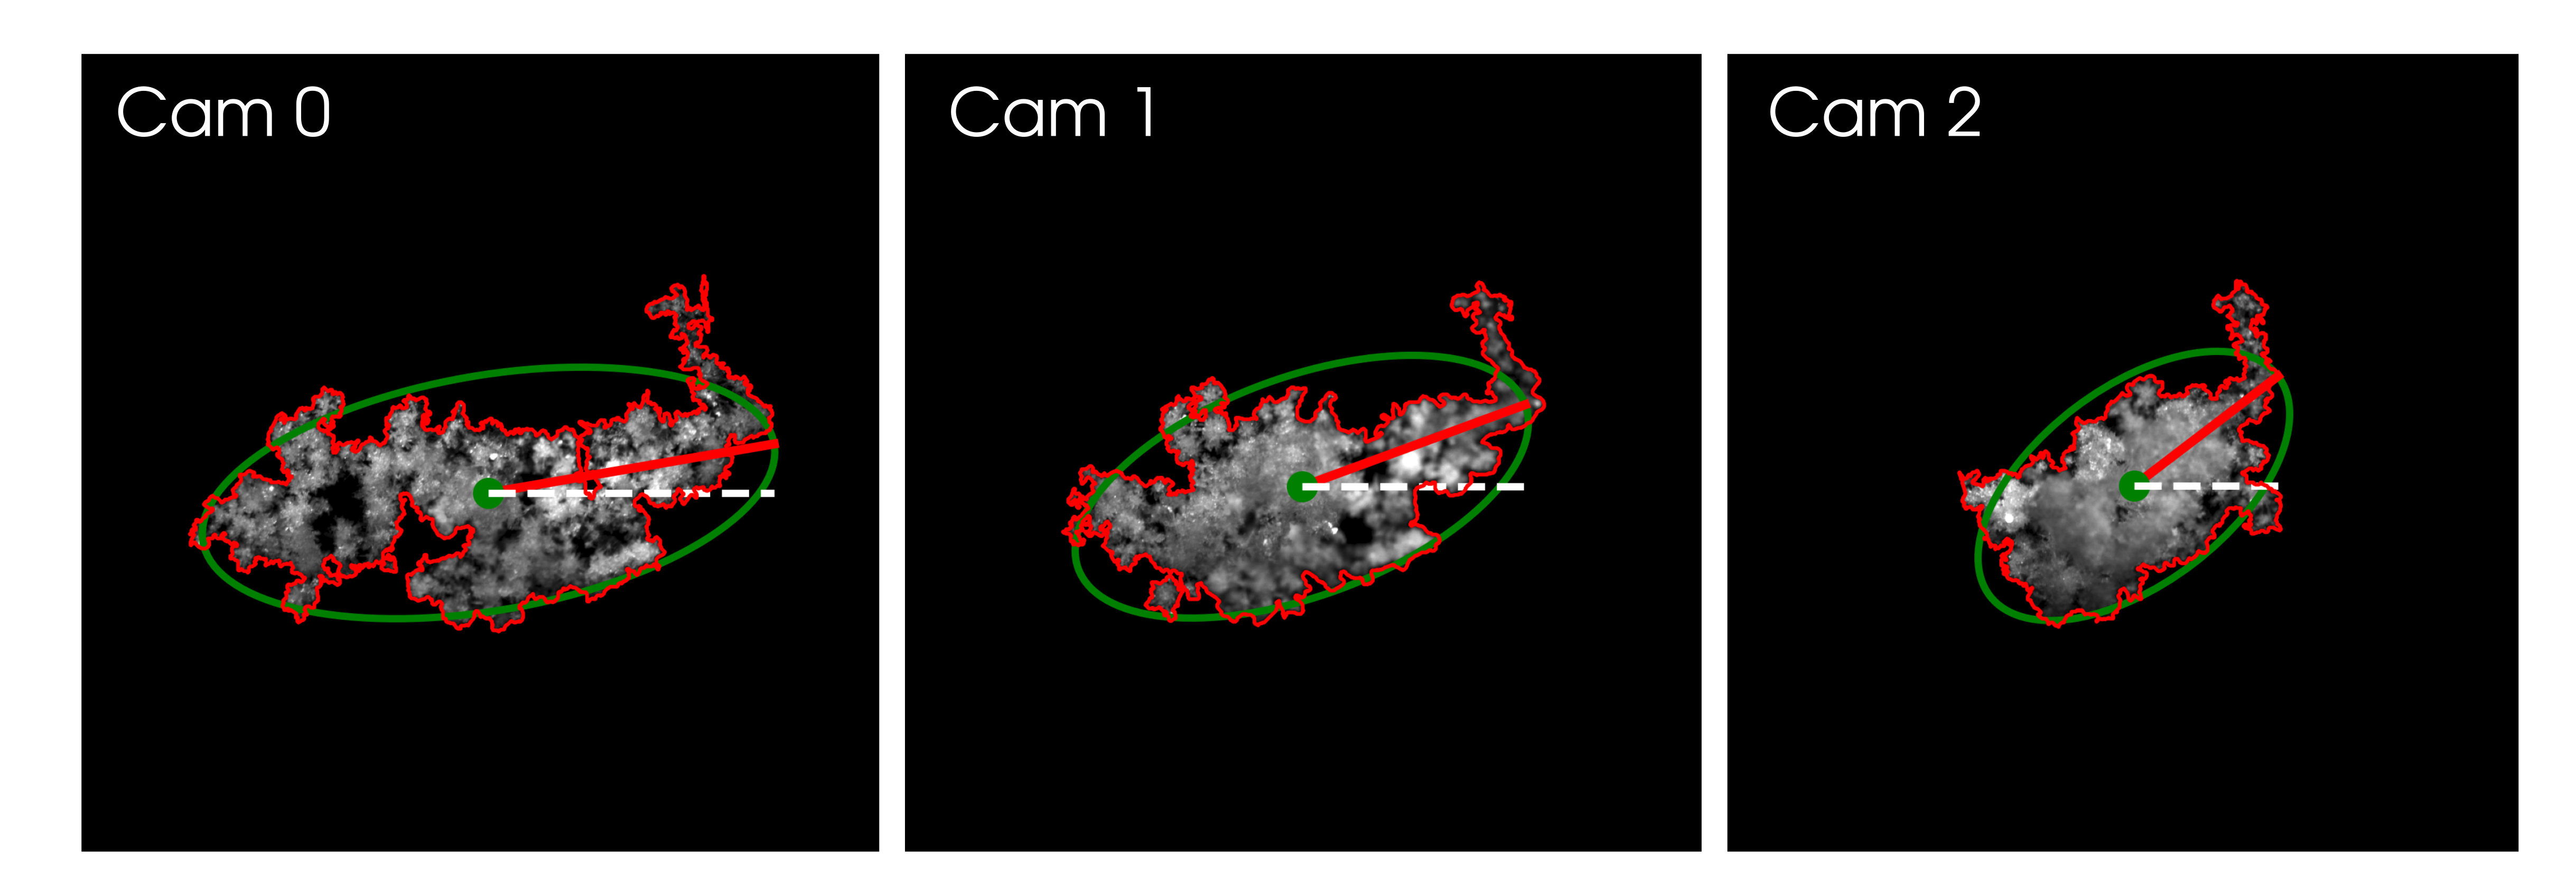
\includegraphics[width=\textwidth]{Fig01.png}
\caption{Example of a triplet of images of a snow aggregate, collected by a MASC. The best fitted ellipse of each image is drawn in green, with the major axis defining the apparent orientation with respect to the horizontal.    }
\label{fig:triplet}
\end{figure}


When handling three 2D images of an individual 3D object, a primary challenge is to derive a single  estimate of orientation for each snowflake. Snowflakes are commonly modeled as ellipsoids or spheroids in previous MASC studies: the orientation of the major axis of the best-fitting ellipsoid in each 2D image is estimated, and the average of the three views is considered as a proxy for orientation \cite{Garrett_GRL_2015, Gergely_JGRA_2016, Fitch_AMT_2021, Fitch_JGR_2022}. The cited studies calculate the mean of the absolute value of the three estimates, an approach referred to here as \textit{Mean\_Abs}. Alternatively, other studies perform a 3D reconstruction of the ellipsoid that best fits all three views and take the orientation of its major axis as the estimate \cite{Jiang_JAS_2019}, a family of approaches named \textit{Ellipsoid\_Fit}. Examining Table~\ref{table:orientations}, the experimental studies using these estimators report the occurrence of non-zero modal orientation values between 10$^\circ$ and 20$^\circ$, challenging the common assumption of a distribution centered at 0$^\circ$. While the non-zero modal values reported for \textit{Ellipsoid\_Fit} in \cite{Jiang_JAS_2019} are based on a small sample of aggregate snowflakes, making evaluation difficult, we demonstrate that the appearance of non-zero modal values in the \textit{Mean\_Abs} approach simply results from averaging absolute values. This will offer a reconciliation between the common assumptions made on hydrometeor orientations and the contradiction of the first studies that used the MASC, a contradiction that was also noted by~\citeA{Garrett_GRL_2015} and discussed in the Conclusions of their work. 

To address this, and to select an appropriate orientation estimator, we conducted numerical simulations (results shown in Fig.~\ref{fig:simulations}). These simulations generated ellipsoids with randomly varying geometries, as well as more realistic and geometrically complex aggregates following the same method as \citeA{Leinonen_AMT_2021}. The objects, of known 3D structure are projected into MASC-like 2D images to test various estimation methods. The orientation of the reference snowflake or ellipsoids is known and drawn from a Gaussian distribution with a zero mean and 25$^\circ$ standard deviation. Although this simulation setup could be expanded extensively to investigate the contribution of each ingredient at play, the goal here is only to support the selection of an estimator to use with actual field-collected data. Figure~\ref{fig:simulations} provides an overview of how various methods reproduce the orientation distribution (panels a and c) and the magnitude of errors relative to the absolute orientation value (panels b and d). Tested estimators include: \textit{Min}, representing the minimum (absolute value) orientation among the views with preserved sign; \textit{Mean\_Abs}, as previously defined; \textit{Ellipsoid\_Fit}, as described; \textit{Mean}, the mean of the estimates from the three views; and individual estimates from each view (\textit{Cam0}, \textit{Cam1}, \textit{Cam2}).

\begin{figure}
 \noindent \centering \includegraphics[width=\textwidth]{Fig02.png}
\caption{Evaluation of the retrieval of orientation that could be achieved with a triplet of MASC images, conducted using simulated data (ellipsoids in the left column, simulated snowflakes in the right column). (a) and (c): distribution of orientation value, both reference and reconstructed. (b) and (d): letter-value plots for the  error distribution of the orientation (in absolute value, not sign dependent). The simulations are conducted on 10'000 ellipsoids of various geometry as well as on 10'000 aggregates. }
\label{fig:simulations}
\end{figure}

The result of the simulations reveal that the non-zero modal values observed with \textit{Mean\_Abs} are artifacts resulting from averaging absolute values, reducing the likelihood of near-zero estimates. With an example: let us assume that the individual estimate of orientation from the three cams were -10$^\circ$, 0$^\circ$ and +20$^\circ$. With \textit{Mean\_Abs} the final estimate would be 10$^\circ$, while for \textit{Mean} it would be 3.33$^\circ$. The results presented here show that, at least statistically-speaking, a bias is introduced. 

The \textit{Ellipsoid\_Fit} method exhibits small errors but its distribution consistently shows a positive bias of a few degrees, making it not centered precisely at 0$^\circ$. Individual camera views yield larger errors and broader distributions, which is in itself a noteworthy result given that many snowflake imagers only capture one view. \textit{Min} provides low errors but produces distributions that are excessively leptokurtic (standardized kurtosis in excess of 5). Consequently, for subsequent analyses, we adopt a straightforward \textit{Mean}, which is possibly an optimal balance between preserving distribution shape, minimal errors and simplicity. \textit{Mean} is the only method in this specific experimental setup that likely maintains Gaussianity,  according to a Kolmogorov-Smirnov test.


\section{Experimental Results and Discussion}
The distribution of \textit{Mean} orientation values in field-collected data, as depicted in Fig.~\ref{fig:alldata}, reveals an overall symmetrical distribution centered at 0$^\circ$. However, the distribution has fat tails with the frequency of large orientation values exceeding the ones of a Gaussian of equivalent standard deviation. The installation conditions of the instruments significantly influence this distribution. DFIR sites show less pronounced tails; in contrast, sites without this artificial sheltering exhibit more pronounced tails and a flatter distribution near 0$^\circ$, ranging between -25$^\circ$ and 25$^\circ$. This suggests that unsheltered observations are likely perturbed by local turbulence induced by the instrument itself, as described in~\citeA{Fitch_AMT_2021}.

\begin{figure}
 \noindent \centering 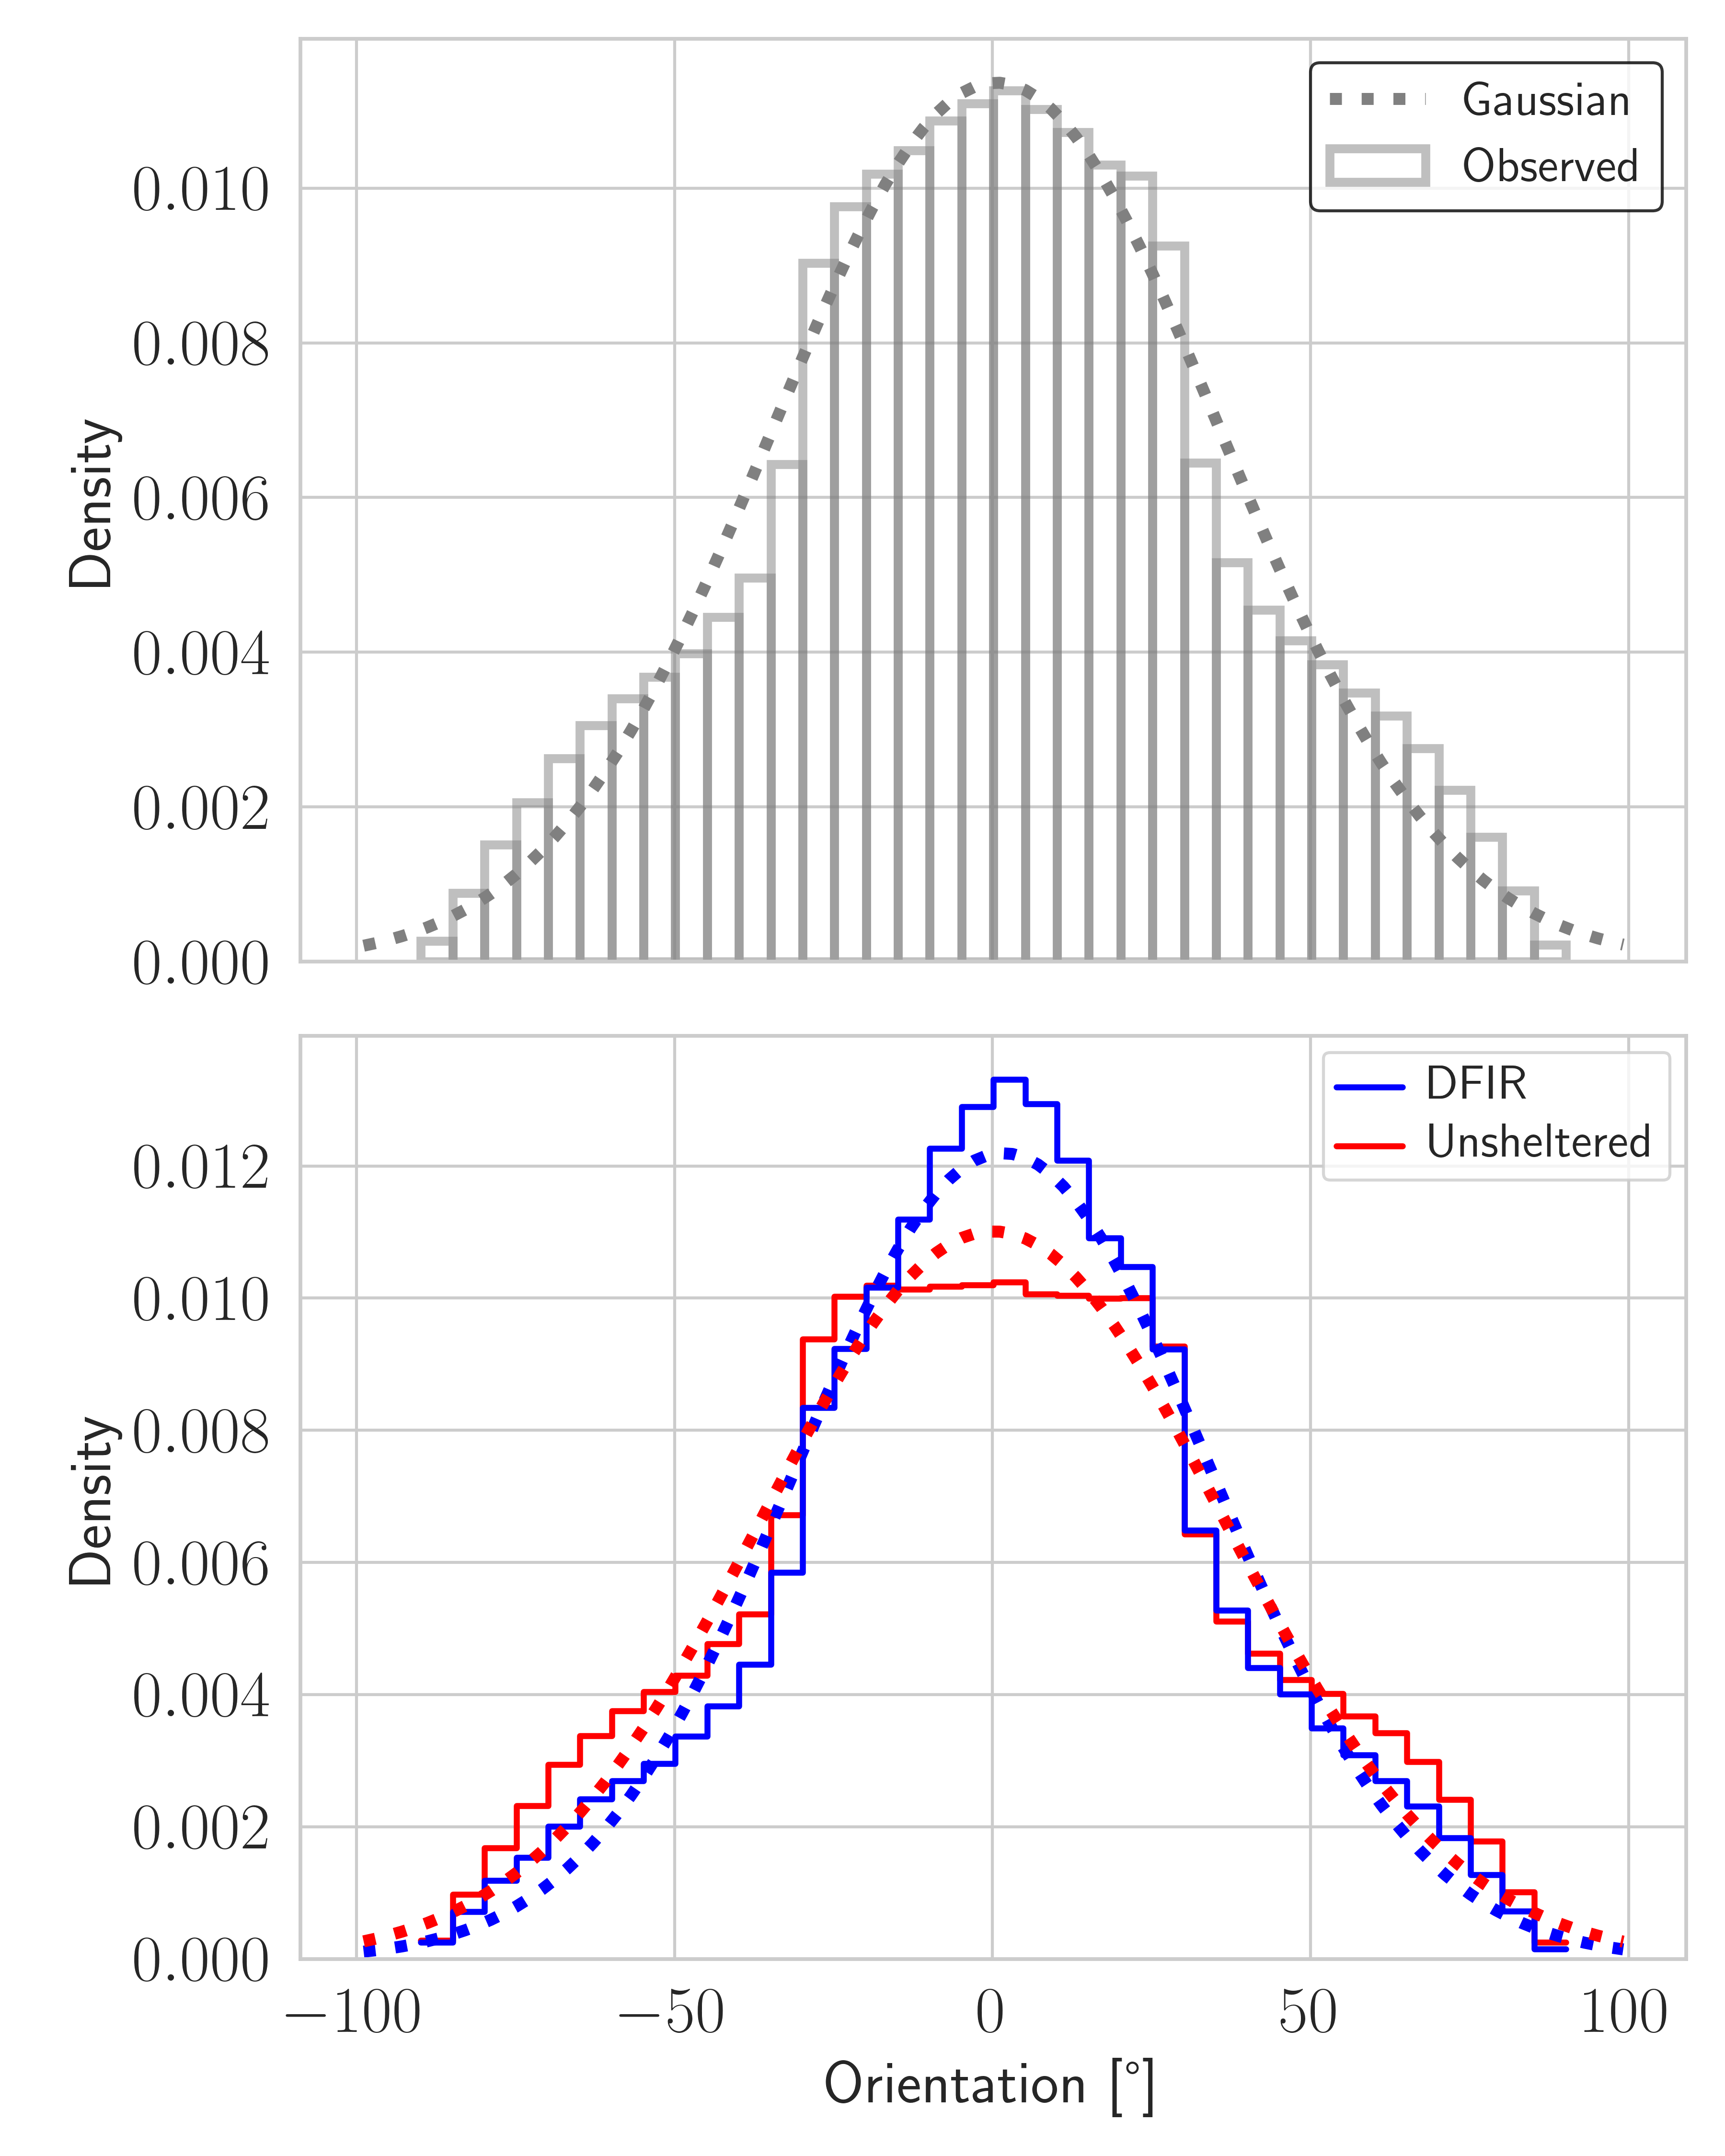
\includegraphics[width=0.8\textwidth]{Fig03.png}
\caption{Histogram of the distribution of orientation value for all data (412'150 particles, top) and data stratified according to the instrumental setup (bottom) either being unsheltered (274'839 particles) or deployed within a double-fence inter-comparison reference (DFIR, 137'311 particles). The dotted lines illustrate the shape of a Gaussian curve having the same mean and standard deviation as the observed data, and are given to provide a visual comparison of the difference with respect to a Gaussian shape (it is not a fit of the histogram). Orientation values are estimated as the sign-preserving mean of the three MASC views.   }
\label{fig:alldata}
\end{figure}

Atmospheric conditions are expected to play a role in shaping orientation distributions: atmospheric turbulence is probably a key driver, as well as horizontal winds interacting with the instrument frame~\cite{Fitch_AMT_2021}. Figure~\ref{fig:wind-effect} compares the standard deviation of orientation distributions between DFIR and unsheltered sites at different wind speeds. At low wind speeds ($<1$ ms$^{-1}$) and high wind speeds ($>10$ ms$^{-1}$), the curves are close. They diverge by up to 5/6$^\circ$ for intermediate wind speeds, with the DFIR curve showing an increase with wind speed once the wind speed exceeds 4 ms$^{-1}$ and being relatively constant below that threshold. Under near-zero wind conditions, local turbulence induced by the instrument  should be minimal, making DFIR and unsheltered conditions comparable. One hypothesis could be that until 4 ms$^{-1}$ the DFIR is effective in minimizing local turbulence (DFIR curve constant, unsheltered curve abruptly increasing), while it gradually loses this capacity until "saturating" around 10 ms$^{-1}$ (DFIR curve increasing, unsheltered curve constant). This interpretation cannot unfortunately tell us any relevant information about the role of environmental turbulence, but only the likely effect of local turbulence introduced by the instrument.  Further research is therefore necessary to clarify these dynamics, in particular the role of natural turbulence in broadening the orientation distribution.

\begin{figure}
 \noindent \centering 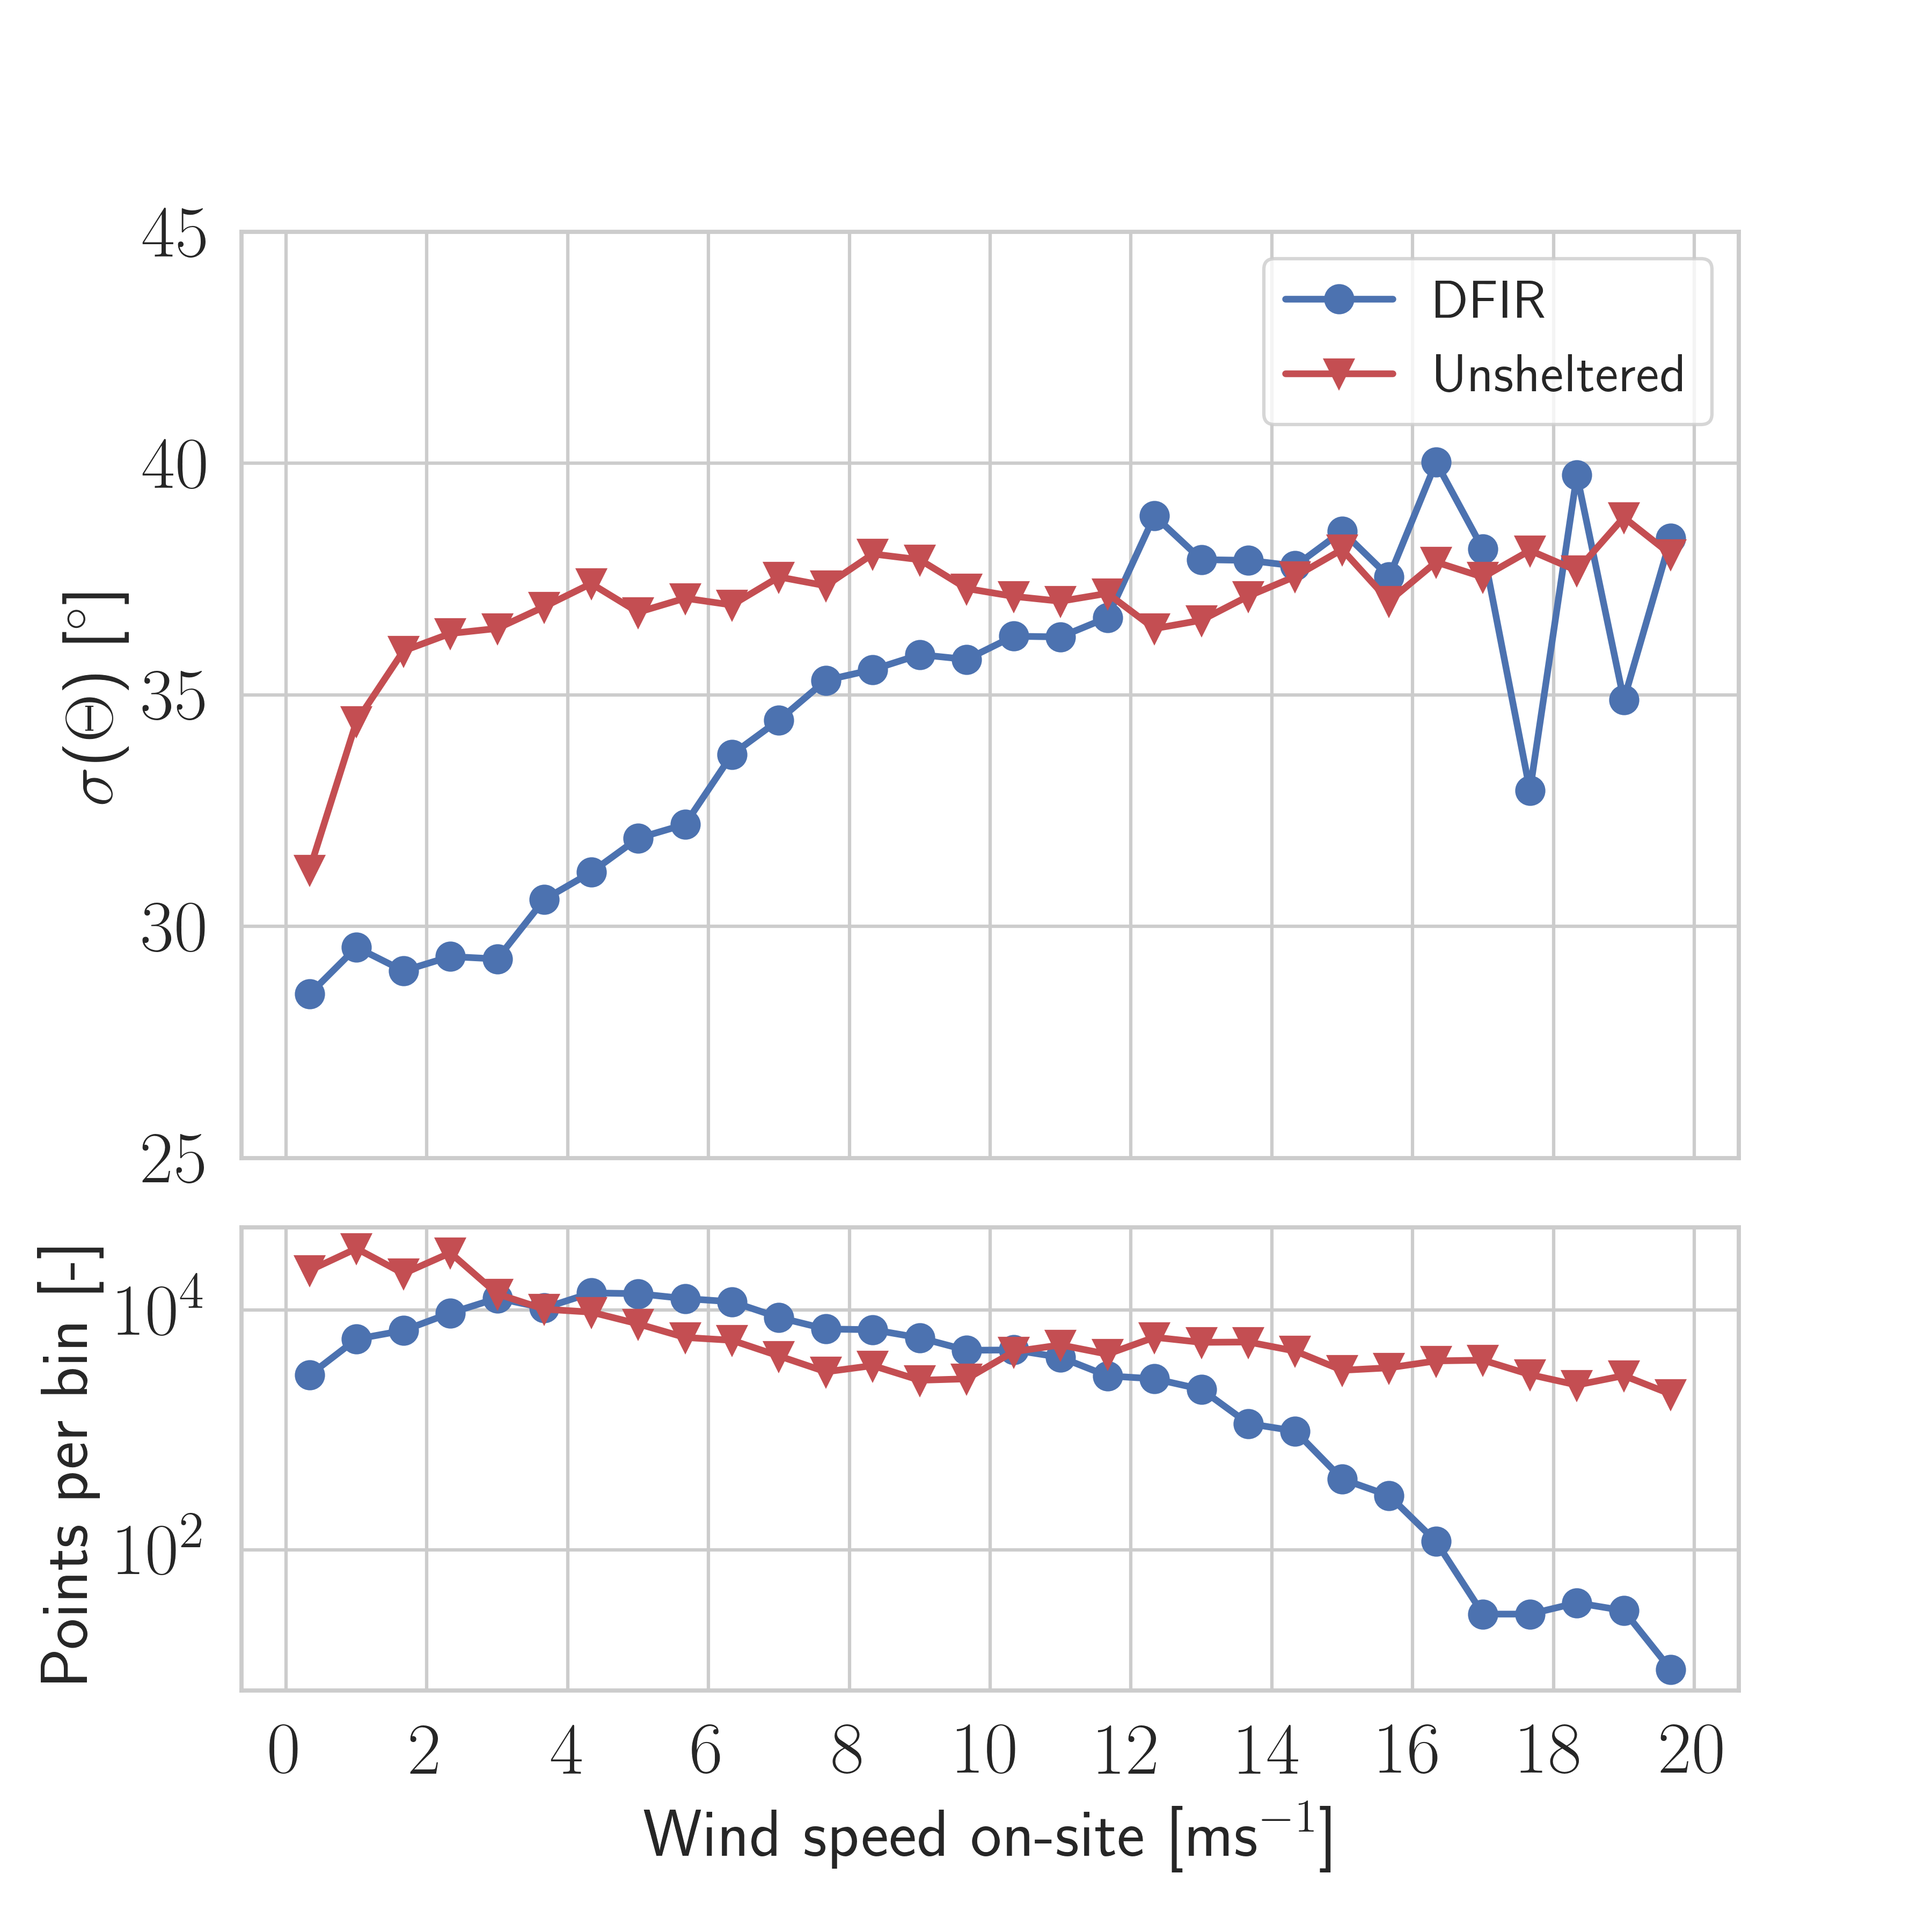
\includegraphics[width=\textwidth]{Fig04.png}
\caption{Evolution of the standard deviation of the  distribution of orientation values at various wind speed levels and stratified according to the instrumental setup. The bottom panel shows the number of observations falling into each bin of wind speed.  }
\label{fig:wind-effect}
\end{figure}

Given that the measurements within DFIRs are less perturbed, we focus now on this siting type. With the original dataset's large size, we can conduct further data stratification and still keep a large data sample. Figure~\ref{fig:hydroclass} illustrates orientation distributions under two contrasting wind regimes ($<4$ ms$^{-1}$ and $>8$ ms$^{-1}$), stratified by hydrometeor type~\cite{Praz_AMT_2017} and average axis ratio. Stronger winds lead to broader and flatter distributions, where a clear mode around 0$^\circ$ orientation values is less evident. For elongated columnar and planar crystals (low axis ratio), this results in distributions showing off-zero modal values, which were not observed under low-wind conditions. A possible explanation is the increasing mean shear with higher wind velocity, which may induce the rotation of suspended particles~\cite{Saffman_JFM_1956}. The results, especially for planar crystal types, must be considered with extreme care. In fact, the classification method of~\cite{Praz_AMT_2017}, which is trained on a supervised set, is able to identify planar crystals when their basal facet is facing towards the MASC cameras, making them recognizable.  This introduces a bias as some orientations would not allow for classification. For example, a thin plate falling perfectly horizontal, would appear in MASC images as a thin column. 

The influence of axis ratio on distribution is not significant, but this is also an important information. It allows to exclude that the observed distribution could be an artefact given by the convention of assigning 0$^\circ$ orientation values to particles with axis ratio of 1. As the shape of the distribution is preserved for low and high axis ratios, we can be confident in the physical nature of this distribution shape. 
 Focusing on low-wind conditions ($<4$ ms$^{-1}$) within DFIR sites, i.e. the subset with minimal external perturbations, the orientation distribution exhibits standard deviations of 28$^\circ$ (graupel), 30$^\circ$ (aggregates), 32$^\circ$ (planar crystals), and 34$^\circ$ (columnar crystals), with a combined value of 29.5$^\circ$ for all types. These values align with commonly assumed ranges (Table~\ref{table:orientations}), yet differ notably from individual studies employing extremely narrow or broad distributions~\cite{Matrosov_JAM_2001, Matrosov_JAS_2005, Ryzhkov_JAMC_2011, Bukovic_JAMC_2018}. Future research should refine these estimates, particularly to discern the impact of actual atmospheric conditions versus instrument-induced effects on distribution shape and breadth.

 
\begin{figure}
 \noindent \centering 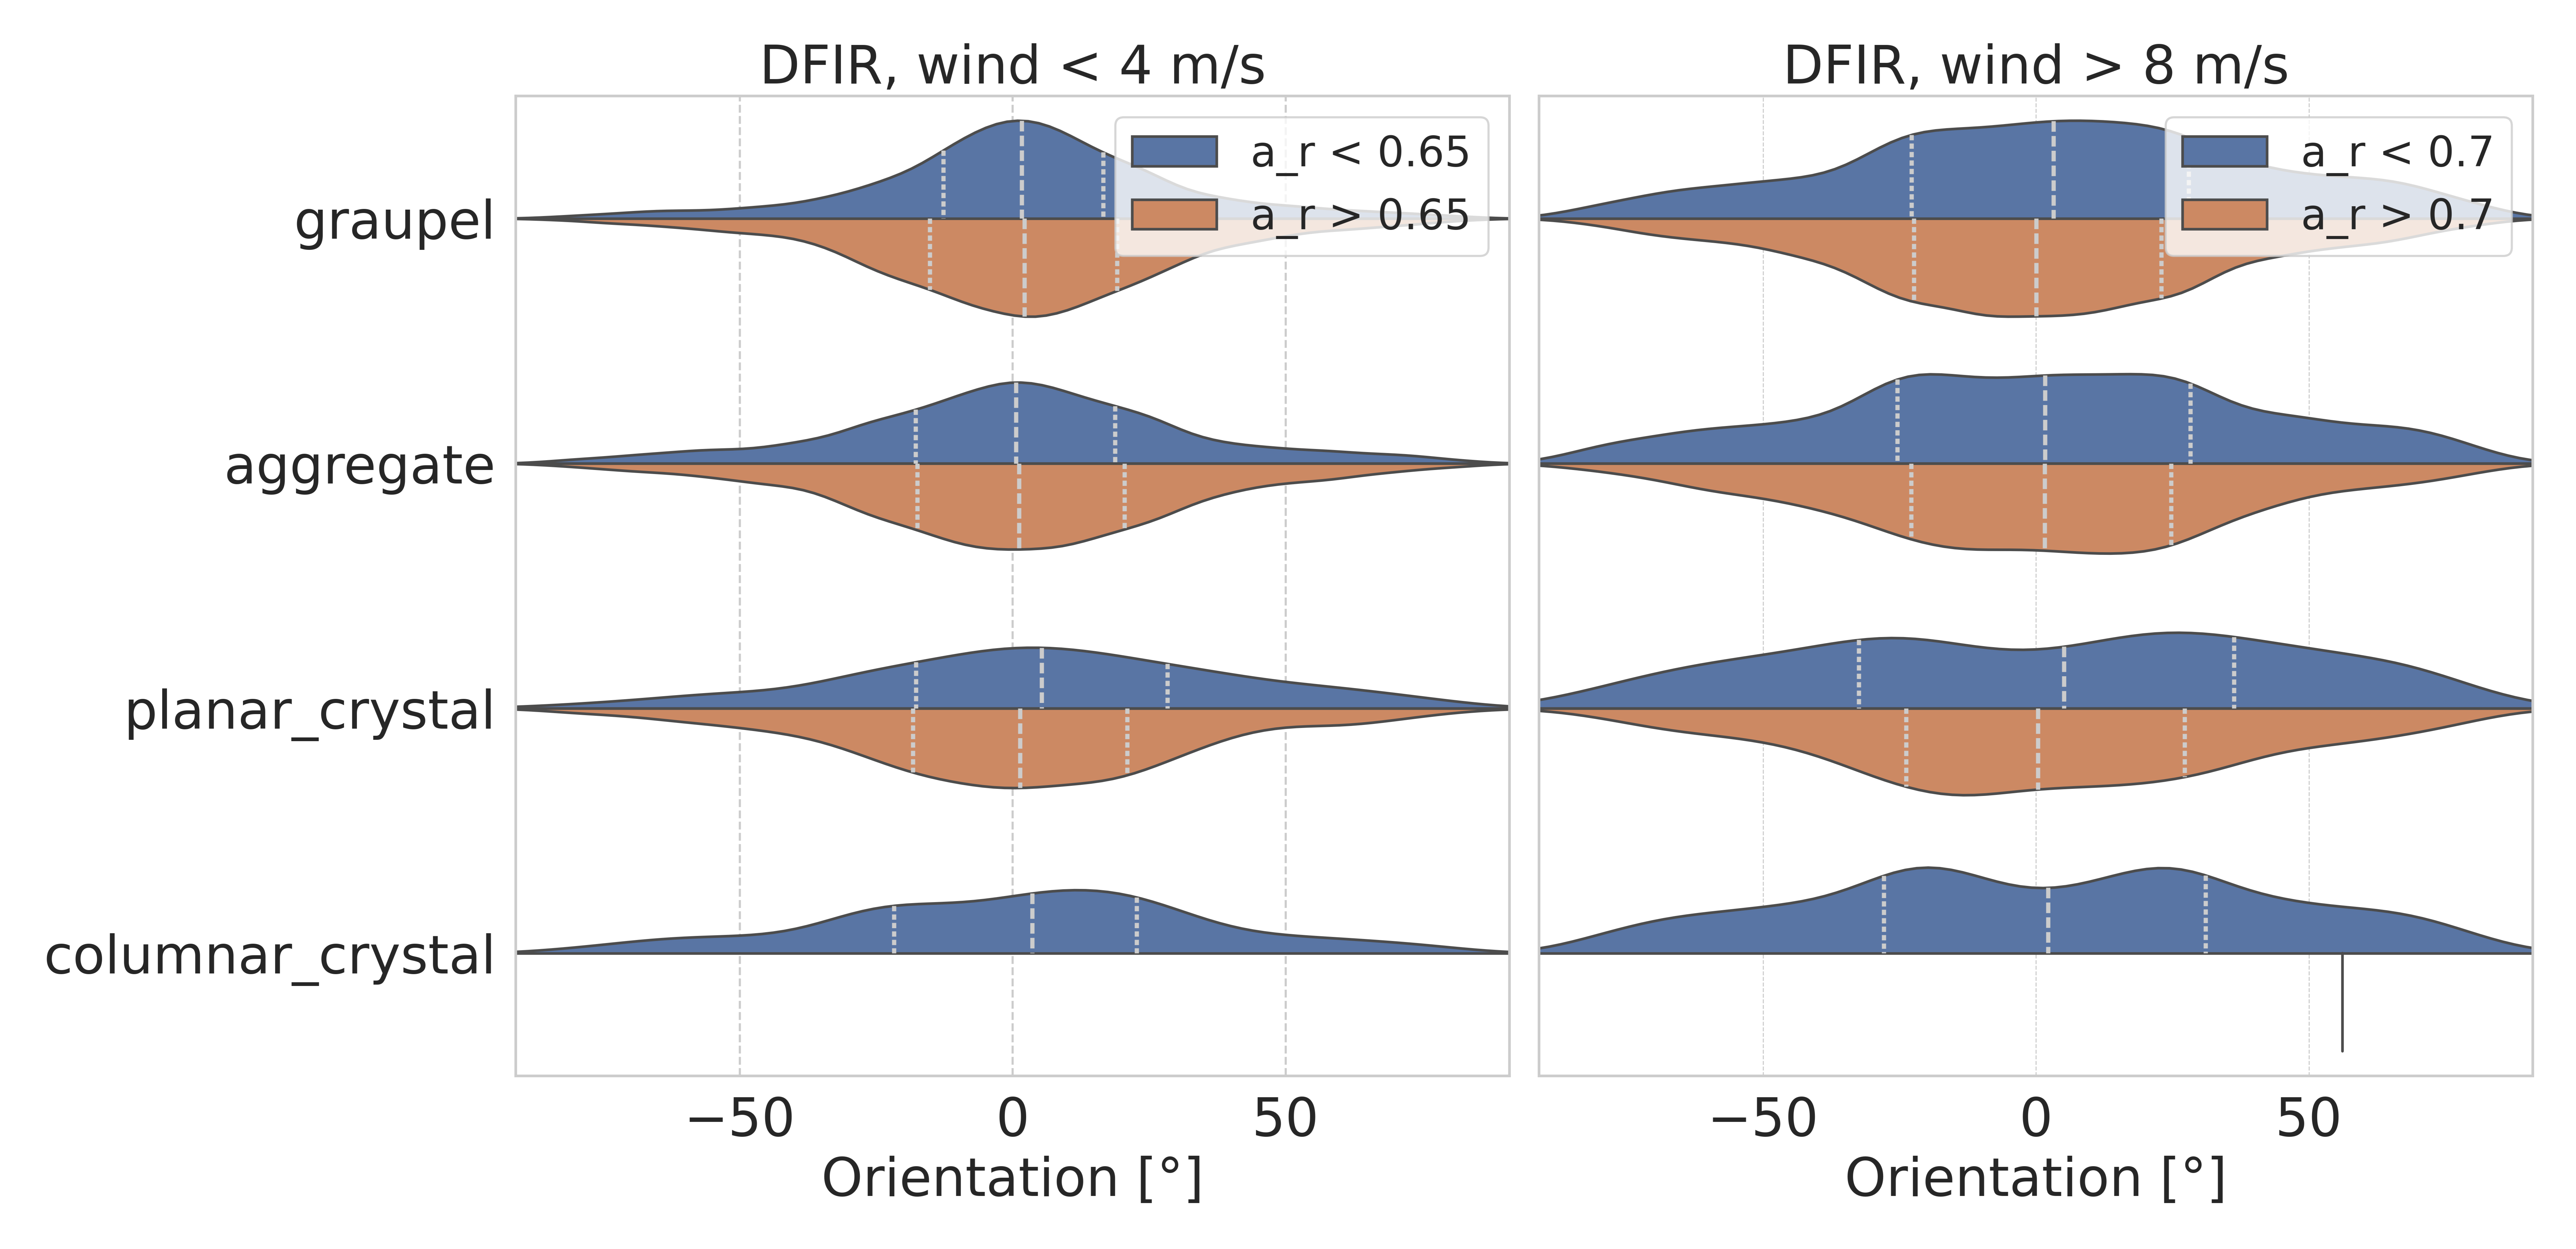
\includegraphics[width=\textwidth]{Fig05.png}
\caption{Violin plot (distribution) of orientation values stratified according to different hydrometeor types. The data correspond to observations collected within a DFIR (Fig.~\ref{fig:wind-effect}), for low horizontal wind (about 47'000 observations for wind $<4$ ms$^{-1}$) and high horizontal wind (about 36'000 observations for wind $>8$ ms$^{-1}$). Data are stratified in two classes of axis ratio (a\_r) limited by the median axis ratio value of the entire population. The number of observations in each distribution ranges between a minimum of 500 (planar crystals, low axis ratio, low wind) and a maximum of about 15'000 (aggregates, low axis ratio, low wind).} 
\label{fig:hydroclass}
\end{figure}


\section{Conclusions}
This study focused on the estimation of the orientation of falling snowflakes using a MASC, providing observational back-up to commonly made assumptions on orientation distributions. It showed how some common data processing choices (for the data processing of MASC data) can lead to biased estimates, and highlighted the effect of unsheltered sites on the collected measurements.
The main results are summarized as follows. 
At first, estimating orientation as the mean of the orientation of the best-fit ellipsoid from each camera view represents a reasonable approach in terms of minimizing errors and accurately reproducing the distribution of (3D) orientation values. Single-camera estimates exhibit high uncertainty compared to combining estimates from all three views and this should be kept in mind if single-view imagers are used. Previous studies reporting median orientations deviating from 0$^\circ$ in MASC studies (in natural outdoor conditions) are likely erroneous because of the artificially non-zero mode resulting from averaging the \textit{absolute value} of orientation estimates from each camera view. This explanation, supported by numerical simulations in the present study, is simpler than what proposed for example by~\cite{Garrett_GRL_2015} who hypothesized fluttering and local, instrument-induced, turbulence (which has anyway an impact) as possible explanations. It must be noted that, at least in quiescent conditions and for some types of planar crystals, spiralling falling modes around a non-zero angle have been observed in the laboratory~\cite{Stout_ACP_2024} but it remains to be seen if this behavior can be observed and isolated also in natural conditions. With this respect, our database is not refined enough to be able to isolate efficiently individual types of planar crystals. 

Field measurements from our large dataset demonstrate that orientation values generally exhibit a symmetrical distribution around 0$^\circ$. Observations from unsheltered sites or in very high wind conditions result in broader and flatter orientation distributions, with a less pronounced mode at 0$^\circ$. This is likely influenced by both local disturbances (instrument-induced) and environmental factors, although with the current information we cannot further decipher the two sources.
It is clear that further research, with different setups is needed to separate the contributions of these effects and estimate the \textit{natural} effect of wind and turbulence on the distribution of orientation values. For this purpose, instruments that do not create local perturbations (like PIP) could be used, ideally co-located with a MASC.   Finally, we observed that orientation distributions of some hydrometeor types can vary significantly with respect to the assumptions made in previous studies.

\section{Open Research}
The MASCDB dataset used to for the field-based data of this study is openly available in~\citeA{MASCDB_dataset_2023}. The scripts to reproduce the results in this manuscript are openly available at this public library:~\url{https://zenodo.org/records/13941866} as well as with codes integrated in the pymascdb package:~\url{https://doi.org/10.5281/zenodo.7398285}.




% Giving latex a width will help it to scale the figure properly. A simple trick is to use \textwidth. Try this if large figures run off the side of the page.








%% SIDEWAYS FIGURE and TABLE
% AGU prefers the use of {sidewaystable} over {landscapetable} as it causes fewer problems.
%
% \begin{sidewaysfigure}
% \includegraphics[width=20pc]{figsamp}
% \caption{caption here}
% \label{newfig}
% \end{sidewaysfigure}
%
%  \begin{sidewaystable}
%  \caption{Caption here}
% \label{tab:signif_gap_clos}
%  \begin{tabular}{ccc}
% one&two&three\\
% four&five&six
%  \end{tabular}
%  \end{sidewaystable}

%% If using numbered lines, please surround equations with \begin{linenomath*}...\end{linenomath*}
%\begin{linenomath*}
%\begin{equation}
%y|{f} \sim g(m, \sigma),
%\end{equation}
%\end{linenomath*}

%%% End of body of article

%%%%%%%%%%%%%%%%%%%%%%%%%%%%%%%%
%% Optional Appendix goes here
%
% The \appendix command resets counters and redefines section heads
%
% After typing \appendix
%
%\section{Here Is Appendix Title}
% will show
% A: Here Is Appendix Title
%
%\appendix
%\section{Here is a sample appendix}

%%%%%%%%%%%%%%%%%%%%%%%%%%%%%%%%%%%%%%%%%%%%%%%%%%%%%%%%%%%%%%%%

%%%%%%%%%%%%%%
% Acronyms
%   \begin{acronyms}
%   \acro{Acronym}
%   Definition here
%   \acro{EMOS}
%   Ensemble model output statistics
%   \acro{ECMWF}
%   Centre for Medium-Range Weather Forecasts
%   \end{acronyms}







%AGU requires an Availability Statement for the underlying data needed to understand, evaluate, and build upon the reported research at the time of peer review and publication.

%Authors should include an Availability Statement for the software that has a significant impact on the research. Details and templates are in the Availability Statement section of the Data and Software for Authors Guidance: \url{https://www.agu.org/Publish-with-AGU/Publish/Author-Resources/Data-and-Software-for-Authors#availability}

%It is important to cite individual datasets in this section and, and they must be included in your bibliography. Please use the type field in your bibtex file to specify the type of data cited. Some options include Dataset, Software, Collection, ComputationalNotebook. Ex: 

\acknowledgments
Jacopo Grazioli has received financial support from the Swiss National Science Foundation (grant no. 200020\_175700/1). 


%% ------------------------------------------------------------------------ %%
%% References and Citations

%%%%%%%%%%%%%%%%%%%%%%%%%%%%%%%%%%%%%%%%%%%%%%%
%
\bibliography{references,references_data}
%
% don't specify bibliographystyle

% In the References section, cite the data/software described in the Availability Statement (this includes primary and processed data used for your research). For details on data/software citation as well as examples, see the Data & Software Citation section of the Data & Software for Authors guidance
% https://www.agu.org/Publish-with-AGU/Publish/Author-Resources/Data-and-Software-for-Authors#citation

%%%%%%%%%%%%%%%%%%%%%%%%%%%%%%%%%%%%%%%%%%%%%%%

%\bibliography{enter your bibtex bibliography filename here}



%Reference citation instructions and examples:
%
% Please use ONLY \cite and \citeA for reference citations.
% \cite for parenthetical references
% ...as shown in recent studies (Simpson et al., 2019)
% \citeA for in-text citations
% ...Simpson et al. (2019) have shown...
%
%
%...as shown by \citeA{jskilby}.
%...as shown by \citeA{lewin76}, \citeA{carson86}, \citeA{bartoldy02}, and \citeA{rinaldi03}.
%...has been shown \cite{jskilbye}.
%...has been shown \cite{lewin76,carson86,bartoldy02,rinaldi03}.
%... \cite <i.e.>[]{lewin76,carson86,bartoldy02,rinaldi03}.
%...has been shown by \cite <e.g.,>[and others]{lewin76}.
%
% apacite uses < > for prenotes and [ ] for postnotes
% DO NOT use other cite commands (e.g., \citet, \citep, \citeyear, \citealp, etc.).
% \nocite is okay to use to add references from your Supporting Information
%



\end{document}



More Information and Advice:

%% ------------------------------------------------------------------------ %%
